\documentclass[11pt,a4paper]{article}
\usepackage{ls}
\usepackage[main=english,russian]{babel}

\newenvironment{code}{\tt \begin{tabbing}
\hskip12pt\=\hskip12pt\=\hskip12pt\=\hskip12pt\=\hskip5cm\=\hskip5cm\=\kill}
{\end{tabbing}}
\def\dq{{\char34}}

\title{About the WUMM modelling concepts of a TRIZ ontology}

\author{Hans-Gert Gr\"abe}

\date{March 22,  2021}

\begin{document}
\maketitle

\section{Background}

In 2019, a group of TRIZ specialists around A.G. Kuryan and M.S. Rubin
launched the \emph{TRIZ Developer Summit Ontology Project} (TOP), to achieve a
review of the status quo and a more accurate ontological mapping of the TRIZ
theory corpus. The work is a natural continuation of earlier efforts by other
authors \cite{TBK2007, TBK2012} to outline a \emph{TRIZ Body of Knowledge}.
While the latter focused on a guide through the literature, TOP is concerned
with the identification of essential concepts and essential relationships
between these concepts using a modern semantic approach. The status of TOP was
presented at the TRIZ Developer Summits in 2019 and 2020 and fixed in two
publications \cite{TOP2019, TOP2020}. In a webinar series\footnote{See
  \url{https://wumm-project.github.io/OntologyWebinar} for links to the
  presentations and an English summary of the talks and discussions.}  first
approaches of a detailed modelling of several sub-areas of TRIZ were
presented.  The project operates its own website
\url{https://triz-summit.ru/Onto_TRIZ/} on which consolidated results are
published.

The main results so far have been a mapping of the continents of the TRIZ
world as a \emph{Top Level Ontology} as well as a (still developing) division
of that world into \emph{Ontomaps} as specifically defined areas, which are to
be modelled in more detail. Moreover, a \emph{thesaurus} of about 500 terms as
essential TRIZ concepts has been identified, which are to be defined more
precisely. The glossary \cite{Souchkov2018} by V. Souchkov in its version 1.2
serves as basis for this work. In the meantime a first list of 100 terms
\cite{TOP-Glossary} has been published on the TOP website.

The efforts differ significantly from earlier approaches to the development of
a TRIZ ontology \cite{Bultey2007, Bultey2015, Cavallucci2011, Dubois2007,
  Zanni2009, Zanni2013}. In those earlier works, the focus was rather on the
modelling of concrete TRIZ analysis steps with the aim to incorporate the
modelling into corresponding tools, e.g. \cite{Cavallucci2011}, or even on the
modelling of processual elements in flow charts, e.g. \cite{Bultey2015}.

The basis for these and the more recent modelling in the TOP project is the
OWL ontology. However, the formal descriptions of logical relationships that
are possible with it -- such as limits for the cardinality of attribute values
of a predicate, which are required to implement of a web interface -- are
expressed in more recent developments of the Semantic Web on the basis of
SHACL, the inference possibilities of OWL that go beyond this are hardly used
in practice, since OWL-Full leads in sufficient generality to provably
undecidable problems, but the modelling restrictions of weaker OWL variants do
not meet the requirements of real-world modelling even of \emph{structural}
relationships in TRIZ.

Our approach therefore returns to modelling based on RDF and consistently
relies on the SKOS ontology as a lightweight framework for modelling
structural relationships in conceptual systems. On this basis we model
\emph{structural} aspects and relationships between TRIZ concepts and tools.
\emph{Processual} relationships as in \cite{Bultey2015} or questions of an
implementation of web interfaces as in \cite{Cavallucci2011} are initially not
covered, although especially for the second question comprehensive experience
from other application areas with the use of SHACL is available. Such a
restriction seems reasonable to us in view of general insights into the
development of conceptual systems \cite{Vygotsky1934} for a first stage of
ontological modelling.

The main disadvantage of the TOP approach so far is the inconsistent use of
semantic means. Such means are used in the background and in the internal
processes of the TOP team, but even a clear namespace concept for
URIs\footnote{URI -- Unique Resource Identifier, one of the basic RDF
  concepts. This string is the \emph{digital identity} of a concept and allows
  to add independently information about «the same thing» in a distributed
  environment. }, the public availability of the results in an RDF store or at
least as files in a relevant format -- all this is missing, not to mention a
SPARQL endpoint for querying the concepts.

However, such an infrastructure was developed and set up in the context of the
WUMM project \cite{WUMM-pages} and used for the representation of actors and
activities of a \emph{TRIZ Social Network}
\url{https://wumm-project.github.io/TSN.html} (persons, conference reports,
presentations, certificates). The data is publicly available in our github
repo \texttt{RDFData} at \cite{WUMM-github} and forms the basis for a
prototypical presentation platform \cite{WUMM-web} that uses simple semantic
tools\footnote{PHP and bootstrap using the EasyRdf PHP library -- the code is
  publicly available in the github repo \texttt{web} at \cite{WUMM-github} for
  study and reuse in own platforms.} to present different facets of the
data. Via a SPARQL endpoint \cite{WUMM-sparql} experts can make their own
complex queries to the dataset.

This technical basis is the starting point for remodelling parts of the TOP
outcome in the course of a \emph{WUMM TRIZ Ontology Companion Project} (WOP)
\cite{WOP}.  This project accompanies the TOP activities in order
\begin{enumerate}[noitemsep]
\item to carry out a remodelling according to semantic standards,
\item to enhance the material multilingually and
\item to build an LOD\footnote{LOD is the abbreviation for \emph{Linked Open
    Data}, a world of interlinked data and «worlds of concepts» steadily
  growing during the last 15 years. See \url{https://lod-cloud.net/}.  }
  infrastructure on this basis,
\end{enumerate}
and thus to improve the basis for the necessary social coordination processes.

In addition to our own modelling (so far of the TRIZ Principles, the TRIZ
Inventive Standards and the TRIZ Business Standards), the \emph{Top Level
  Ontology} and the division into \emph{Ontomaps} are available in this
format. The work on a \emph{thesaurus} as well as the presentation of
different approaches to a common glossary is actively accompanied. In the WOP
approach the differing definitions of different TRIZ schools can coexist more
clearly side by side than it is conceptually possible (and is probably not
aimed at) in the TOP approach. This aspect, together with the focus on
multilinguality, for which individual translation projects can easily be
delimited based on the relevant RDF concepts, represent the essential
additional contributions of the WOP approach.

The aim of this paper is to explain the basic modelling and semantic
assumptions, concepts and settings of the WOP approach in more detail. 

\section{Modelling a TRIZ ontology}

\subsection{TRIZ and the World of (Technical) Systems}

All TRIZ concepts revolve around the central notion of a \emph{system}, its
planning, creation, operation, maintenance, further development, etc.
Following the widely accepted understanding of that concept in the TRIZ
community, TOP defines
\begin{quote}
  A \emph{system} is a set of elements in relationship and connection with
  each other, which forms a certain integrity, unity. The need to use the term
  «system» arises when it is necessary to emphasize that something is large,
  complex, not fully immediately understandable, yet whole, unified. In
  contrast to the notions of «set» and «aggregate», the concept of a system
  emphasises order, integrity, regularities of construction, functioning and
  development. The notion of system is part of the system and functional
  approach, and is used in the system operator.
\end{quote}
Usually, however, the definition of a system refers to the concept of a
\emph{component}, as in Souchkov's glossary \cite{Souchkov2018}:
\begin{quote}
  \emph{Technical System:} A number of components (material objects) that were
  consciously combined to a system by establishing specific interactions
  between the components. A technical system is designed, developed,
  manufactured, and assigned to perform a controllable main useful function or
  a number of functions within a particular context. A technical system can
  include subsystems which can be considered as separate technical systems.

  \emph{Component:} A material object (substance, field, or substance-field
  combination) that constitutes a part of a technical system or its
  supersystem.  A component might represent both a single object and a group
  of objects.
\end{quote}
We thus conclude that a system is essentially a collection of components that
interact in a specific way to produce the characteristic functionalities of
the system.  The subsystems referred to as components provide own functions
for this, but the functionalities of the system do not result from a simple
addition of the component functions, but as an emergent system property from
their interaction. For the modelling of systems, their structural organisation
(the «machine» in the sense of \cite{TT}) and their workflow organisation
(«how the machine works», ibid.)  are equally important.  The systemic
approach is thus self-similar and fractal; the terms «system» and «component»
are largely used synonymously depending on the respective \emph{modelling
  focus}.

In TRIZ, an \emph{engineering problem} is always conceptualised as the design
of a new system or the improvement of an existing one. We regard the design of
a new system as a special case of further development, since in this case,
concepts of a model of the «system as it is» do exist, how vague they may be.

The delimitation of meaningful systems as modelling units has many facets and
points of view, see for example \cite[section 8]{Szyperski2002}. In the TRIZ
concepts, a certain functional completeness plays a major role in this
delimitation, even if a defined throughput of energy, material and information
is required for its operation.  For a system, its \emph{design} and
\emph{operation} have to be distinguished, as explained in more detail in
\cite{Graebe2020}. This also applies to \emph{components} of a system.  In the
white-box analysis of a system, its components are considered as working
black-boxes, which are characterised in the design dimension by a
\emph{specification of their functionality} and in the operation dimension by
the \emph{guaranteed specification compliant operation}, provided that the
operating conditions (in particular the throughput of material, energy and
information required for its operation) are ensured within the system. The
description of these operating conditions is part of the specification, which
thus consists of an input and an output part (also referred to as import and
export interfaces).

The components thus constitute a \emph{world of technical systems} in the
sense of the explanations in \cite{Graebe2020}, to which we refer for further
details of this conceptualisation.

\subsection{Abstraction Levels of Modelling}

An ontology is about «modelling of models», because the clarification of terms
and concepts aimed at with an ontology is intended to be practically used in
real-world modelling contexts.  This «modelling of models» references a
typical engineering context, in which the \emph{modelling} of systems plays a
central role and serves as basis of further planned action (including project
planning, implementation, operation, maintenance, further development of the
system).

In this process, \emph{several levels of abstraction} are to be distinguished.
\begin{itemize}[noitemsep]
\item [0.] The level of the \emph{real-world system} to which the engineering
  task refers. This level is only \emph{practically} accessible. The model to
  be developed at level 1 must be appropriate to cover all problems arising in
  the process of development and use of the system and express the inherent
  contradictoriness of the system.

  This contradictory nature of the system can be formulated only in language
  form, i.e. on the model level and \emph{applying} the concepts available
  there.  These concepts must therefore not only be able to describe the
  system itself, but also cover a description of the necessary aspects of its
  operation.
\item[1.] The level of \emph{modelling the real-world system}. In the
  modelling of a real-world system with its "core and cross-cutting concerns"
  (as known from Software Engineering), the worlds of several conceptual
  systems often come together. In addition to the methodological dimension of
  a TRIZ ontology, these are regularly the conceptual world of a technical
  ontology and possibly other conceptual worlds such as a company-internal
  compliance etc.

  The ontologies provide the language means, concepts (RDF subjects) and
  properties (RDF predicates), which are to be \emph{applied} at this level.
  This level is also the \emph{level of methodological practice}.
\item[2.] The \emph{level of the meta-model} as the actual (TRIZ) ontology
  level on which the systemic concepts are \emph{defined}. This definition is
  processed \emph{applying} the methodological concepts whose linguistic means
  are made available on meta-level 2.
\item [3.] The \emph{modelling meta-level 2} at which the methodological
  concepts are defined.
\end{itemize}

\subsection{The TOP Concept of a System}

A central concept in TOP modelling is the distinction between the stages of 
\begin{itemize}[noitemsep]
\item [(1)] the system as it is,
\item [(2)] the TRIZ model of the system as it is,
\item [(3)] the TRIZ model of the system as required, and 
\item [(4)] the system as required. 
\end{itemize}
The TOP glossary \cite{TOP-Glossary} explains the differences as follows
\begin{itemize}[noitemsep]
\item [(1)] The \emph{system as is} is a system in its original state before
  it is analysed and transformed into a new «system as is».
\item [(2)] The \emph{TRIZ model of the system as is} is formed from the
  «system as is» by means of various TRIZ models: component-structural and
  functional models, su-field or ele-field models, description of
  contradictions or of typical conflict schemes, etc. Depending on the chosen
  model type, the model will be transformed into the «TRIZ model of the system
  as required».
\item [(3)] The \emph{TRIZ model of the system as required} is formed from the
  «TRIZ model of the system as is» by procedures which correspond to the
  selected model transformation method (functional, su-field, ele-field,
  solution of the contradictions in requirements and properties, etc.). The
  transition is performed along the line
  \begin{center}
    «System as is» $\to$ «TRIZ model of the system as is»\\ $\to$ «TRIZ model
    of the system as required» $\to$ «System as required»
  \end{center}
  in accordance with the scheme of a TRIZ Model.
\item [(4)] The \emph{system as required} is a system derived from the «system
  as is» through a transformation, based on the «model of the system as
  required».
 \end{itemize}
It is clear that "system" here can only mean a \emph{model of the system} in
which, in addition to the ontology of the TRIZ methodology, a domain-specific
ontology plays a central role, because a system is only accessible in
descriptive terms via its model, as the schematisation in Figure~1 also
suggests.
\begin{center}
  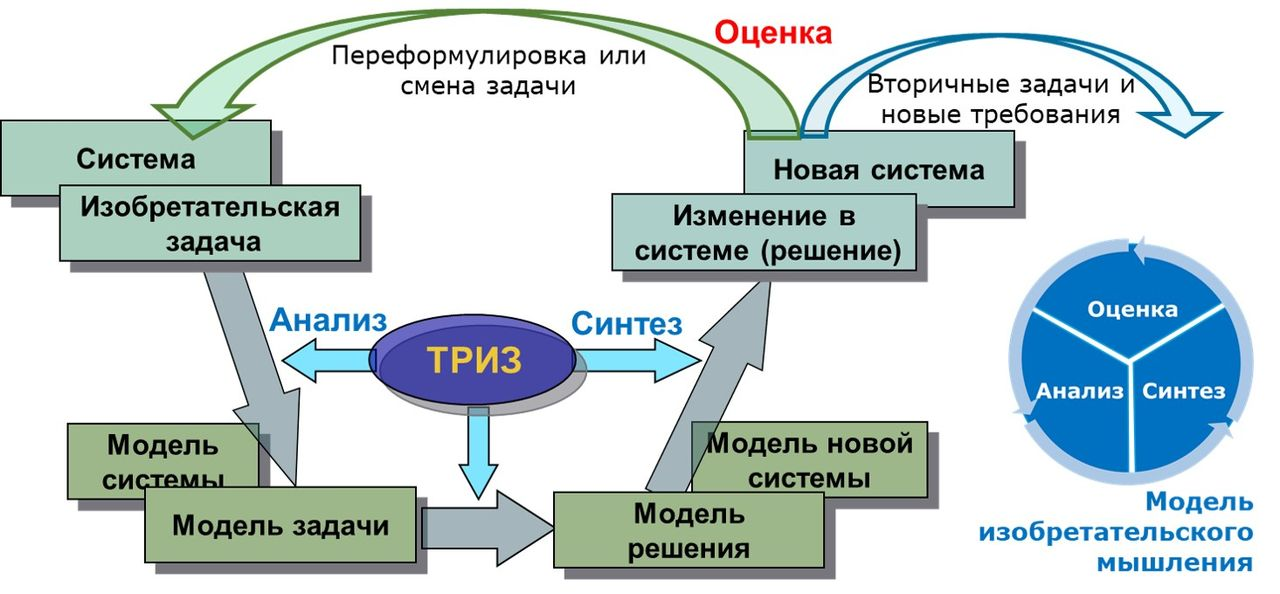
\includegraphics[width=.6\textwidth]{Rubin.jpeg}\\
  Figure 1. Visualisation of the TOP TRIZ model.
  \url{https://triz-summit.ru/onto_triz/mod}
\end{center}
What is a \emph{TRIZ model} as defined in the TOP project?  This notion ist
explained in \cite{TOP-Glossary} as follows:
\begin{quote}
  A \emph{TRIZ model} is a schematic notation of a gradual transition from the
  problem to TRIZ model of the problem, then to TRIZ model of the solution and
  then to the solution itself; or from the system to TRIZ model of the system,
  then to TRIZ model of the new system and then to actual change of the system
  («system as required»). The TRIZ model includes the basic components of
  inventive thinking: analysis, synthesis, evaluation.
\end{quote}
In contrast to the above explanations, here a TRIZ model is understood as the
totality of the four model stages described above, including the modelling
process itself. However, these four stages all refer to level 1 models of a
real-world system; no distinction is made between application of concepts from
level 2 of a \emph{TRIZ ontology of tools} (present at level 1 as concept
instances) and level 3 of a \emph{TRIZ ontology of methods} (present at level
1 only in a methodological-processual way).

What is the core of the three transitions between the model stages?  The
modelling of any system starts with the modelling of the «system as it is» on
the basis of domain-specific concepts. If the modelling is done on the
methodological basis of TRIZ principles, the domain-specific system of
concepts must be enriched with TRIZ methodological concepts such as main
useful function, conflicting pairs, operative zone and operative time, etc.,
in order to prepare the extraction of abstract TRIZ patterns as «TRIZ model of
the system as it is» (TRIZ task model) according to the hill model. This part
of the TRIZ ontology concerns thus only \emph{one} aspect of the modelling of
the real-world system. On the other hand, the \emph{application} of TRIZ
concepts in such a real-world modelling requires that the domain-specific
concepts are compatible with the requirements of TRIZ modelling. However, the
real-world modelling has a similar relationship of the specific to the general
of a domain-specific ontology as to a TRIZ ontology. Thus, the two ontologies
stand in a relationship of mutual complementation of the modelling languages
in the special modelling application.

It is clear, however, that the «model of the system as it is» (MSI) enriched
with elements of a domain-specific ontology, the abstract «TRIZ model of the
system as it is» (TSI) extracted from it, the resulting «TRIZ model of the
system as required» (TRIZ solution model, TSO) and finally the «model of the
system as required» (MSO), which is again enriched in a domain-specific way,
call up largely the same language constructs from the point of view of a TRIZ
ontology and are thus four instances of the real-world system model, which are
related as follows:
\begin{itemize}[noitemsep]
\item \textbf{MSI $\to$ TSI:} Consolidation and refinement of TRIZ-relevant
  concepts in the MSI.
\item \textbf{TSI $\to$ TSO:} Description of an abstract transformation and
  execution of the parts of the transformation that are possible at this
  level, i.e. without interaction with the domain-specific modelling.
\item \textbf{TSO $\to$ MSO:} Detailing of the model, completion and execution
  of the domain-specific part of the transformation.
\end{itemize}
For the Level 2 ontology (it answers the question "Which TRIZ tools are
available and how do they relate to each other?"), the distinction between
these four system models is therefore not relevant. Corresponding language
tools are only needed at level 3, when it comes to the terminology of the
\emph{application} of the TRIZ methodology itself.

Concerning the balance between the new and the old, as suggested by relevant
methodologies for the further development of conceptual systems, we see the
need to clearly distinguish between these two levels of ontologisation and
limit our ontological modelling to level 2.

\section{Basics of the WUMM Ontology Project}

\subsection{SKOS Basics}

The SKOS ontology allows to express concepts and their relations in a
lightweight way. The class \texttt{skos:Concept} and the predicates
\texttt{skos:narrower}, \texttt{skos:broader} and \texttt{skos:related} are
used for this purpose. The first two predicates describe hierarchical
relationships between concepts\footnote{From the SKOS Primer
  \cite{SKOS-Primer}: «The subject of a \texttt{skos:broader} statement is the
  more specific concept involved in the assertion and its object is the more
  generic one», i.e. \texttt{A skos:broader B} expresses that A is a
  subconcept of B.  \texttt{skos:narrower} is the inverse property to
  \texttt{skos:broader}.}, the third is used for non-hierarchical
relationships.

Relationships between concepts can be of very different structure.
Hierarchical relationships, for example, can model (transitive) subconcept
relationships in taxonomies as well as whole-part relationships, which are
inherently non-transitive when concepts of different qualities are related.
Both types of conceptualisation have an intentional as well as an extensional
aspect -- the new units of meaning, especially their emergent properties, can
neither be adequately described by mere enumeration of their subconcepts nor
by the «legitimate interpretation of sense» of the purposes of their
constitution in the sense of \cite{BergerLuckmann}. In the SKOS primer
\cite{SKOS-Primer} these modelling aspects are described in more detail,
especially the modelling of class-instance and whole-part relationships. We
follow the recommendation in \cite[Sect 4.7]{SKOS-Primer} and introduce
subpredicates of the generic SKOS predicates listed above for different
modelling contexts. More detailed modelling rules for such contexts are
described and discussed below.

Since this project is about modelling a unified space of TRIZ concepts,
further SKOS aggregation concepts such as \texttt{skos:ConceptScheme},
\texttt{skos:Collection}, \texttt{skos:OrderedCollection} etc. are not used.
The aggregation of different concepts in collections (assignment to TRIZ
generations \cite[Table 1]{TOP2020} or in concept classes \texttt{Basic},
\texttt{Model}, \texttt{Rule} and \texttt{TermGroup} \cite[Fig. 4]{TOP2020})
is realised via special predicates.

We use the SKOS ontology \cite{SKOS} with the concepts (K)
\begin{itemize}[noitemsep]
\item \texttt{skos:Concept}, \texttt{skos:prefLabel}, \texttt{skos:altLabel}
  -- concept naming
\item \texttt{skos:definition}, \texttt{skos:example}, \texttt{skos:note} --
  concept properties
\item \texttt{skos:narrower}, \texttt{skos:broader}, \texttt{skos:related} --
  concept relations.
\end{itemize}
SKOS provides an initial descriptive framework for conceptualisations.  For
the meaning of the individual concepts, we refer to \cite{SKOS} and the
explanations below.

\subsection{URIs and Namespaces}

One of the central problems of transferring the existing data stocks on TRIZ
concepts is the allocation of meaningful URIs, since the individual glossary
entries in the existing TOP sources are identified solely by their labels.
The OSA platform\footnote{The OSA platform is used as an TOP internal ontology
  editor, see \url{https://wumm-project.github.io/TOP} for more information
  about the platform, its odds and evens.} is no exception to this since the
URIs assigned there (both for the nodes and the edges of the constructed RDF
graph) are not publicly visible.

One of the first decisions that must be made for the allocation of URIs is the
\emph{definition of namespaces} that correspond to the different modelling
contexts. Since an \emph{ontology modelling} basically has the purpose of
being applied in \emph{modellings of real-world systems}, at least these two
modelling contexts have to be distinguished. The modelling context of a
(prototypical) real-world system will usually only play a role in examples in
which the effect of ontology modelling decisions is practically demonstrated.
At the level of ontology modelling, we further distinguish between the parts
of the concepts that are largely uncontroversial\footnote{These are mainly the
  \emph{concepts} to be included in a glossary. We assign URIs of a
  \texttt{skos:Concept} to them and model their names as
  \texttt{skos:prefLabel}.} and the parts of the concept for which special
conceptual approaches have been developed within the WUMM Ontology Project
(WOP).  For these different abstraction layers we use the following
namespaces:
\begin{itemize}[noitemsep]
\item \texttt{ex:} -- the namespace of a special system to be modelled. 
\item \texttt{tc:} -- the namespace of the TRIZ concepts (RDF subjects).
\item \texttt{od:} -- the namespace of WUMM's own concepts (RDF predicates,
  general concepts). 
\end{itemize}

During the computer based transformation of the datasets into a valid RDF
format, a first suggestion for URIs in the namespace \texttt{tc:} was
automatically generated and then further consolidated in several steps. An
essential task still to be done is to finish this final consolidation of URIs,
i.e. to merge URIs generated from different sources that refer to the same
concept.

\subsection{Provenance of Explanations}

Another problem of this ontological modelling is the representation of the
provenance of the individual explanations. For this purpose the SKOS concepts
listed under (K) were replaced for each individual source by notations from
the namespace \texttt{od:} in order to address the «worlds» of the individual
TRIZ schools separately.  The same applies to the use of provenance-dependent
subclasses of \texttt{skos:Concept}.

Such notational variations are for example
\begin{itemize}[noitemsep]
\item \texttt{skos:Concept} $\to$ \texttt{od:GSAThesaurusEntry},
  \texttt{od:VDIGlossaryEntry} \ldots
\item \texttt{skos:definition} $\to$ \texttt{od:SouchkovDefinition},
  \texttt{od:VDIGlossaryDefinition} \ldots
\item \texttt{skos:example} $\to$ \texttt{od:VDIGlossaryExample} \ldots
\end{itemize}
etc.  Here \texttt{GSAThesaurus} stands for the thesaurus published on the
Altshuller website \cite{GSA}, \texttt{VDIGlossary} for the VDI glossary
\cite{VDI} and \texttt{SouchkovDefinition} for the glossary
\cite{Souchkov2018} by V. Souchkov. All these data were available or provided
to the WUMM project in a machine-readable format, transformed by us into
suitable RDF formats and are available as open source both as files in the
github repo \texttt{RDFData} at \cite{WUMM-github} and in our RDF Store
\cite{WUMM-store}. See the RDF data itself, which can also be queried via our
SPARQL endpoint \cite{WUMM-sparql}.

This can be used to build a \emph{combined glossary} where definitions from
different TRIZ schools of the same concept co-exist. This is implemented
prototypically\footnote{Seee \url{http://wumm.uni-leipzig.de/ontology.php}.}
im such a way, that for each concept represented by a URI, a link displays all
RDF triples in which this concept occurs as a subject or object. Further links
in this representation can be used to navigate in the entire RDF graph (more
precisely: in its respective connected component).

\subsection{Modelling Systems and TOP TRIZ Models}

Since TOP system models in (1) and (4) come with additional modelling
information based on a great variety of domain-specific ontologies the TRIZ
ontology is an add-on only and (domain-specific) ontology integration
engineering approaches are required anyway. It is thus justified to
concentrate solely on the concerns of modelling the TRIZ-relevant aspects in
all four modelling stages.

In the TOP approach, the distinction of these modelling stages is consistently
introduced for all system-relevant concepts at the level of subconcepts.
However, since the transition from one modelling stage to the next is carried
out jointly for all concepts related to the system, it is sufficient to assign
the modelling stage to the respective model of the system as a property.
Separate sub-concepts at all levels, as introduced in TOP modelling, are not
necessary, since the stage can be inferred via the model of the system in
which a concept is "built in". Hence the WOP approach takes a different route
here and models this connection as a predicate \texttt{od:belongsTo} with
value from the \texttt{tc:StageValue} range
\begin{center}\tt
  tc:SystemAsIs, tc:SystemAsRequired, tc:ModelAsIs, tc:ModelAsRequired
\end{center}
to assign to a concept \emph{instance} in a real-world modelling one of the
modelling stages as discussed above.  This also makes it easy to extend the
\texttt{rdfs:range} of this property if, for example, stages of earlier or
later system versions are to be included in the modelling of a special system
in the context of an application of the system operator.

This significantly reduces the number of concepts to be distinguished, which
is also indicated by reasons of homogeneity, since the different stages of
this system model must be structurally similar in order to be able to capture
structural continuities within its development, and thus must be modelled by a
single uniform concept.

\section{Typical modelling situations}

\subsection{Class-instance relation}

In OO programming classes are usually extensionally conceptualised as a
concept of member functions and attributes that are common to all instances of
that class.  We do not consider here the special possibility to define also
static attributes and functions for a class.  In this sense the class concept
generalized the concept of its members.  A special way to conceptualize
classes with a finite number of instances are \emph{morphological tables}.

Within the WOP approach this relation is modelled using the predicates
\texttt{od:allowedValues} (a subproperty of \texttt{skos:narrower}) and
\texttt{od:valueOf} (a subproperty of \texttt{skos:broader}). The class
concept belongs to the WOP category \texttt{od:PropertyDomain}. No distinction
is made between attribute (left column of a morphological table) and the
attribute value range (set of values in the right column of a morphological
table).

\emph{Example:}  Colour (red, green, yellow, blue).

\begin{code}
  ex:MeiersCar a ex:Car; od:hasColour tc:green . \\[4pt]
    
  od:hasColour a rdfs:Property;\\
    \>rdfs:domain ex:Car;\\
    \>rdfs:range tc:Colour .\\[4pt]

  tc:Colour a skos:Concept, od:AdditionalConcept ;\\
  \>skos:prefLabel {\dq}Colour{\dq}@en, {\dq}Farbe{\dq}@de ;\\
  \>od:WOPCategory od:PropertyDomain ;\\
  \>od:allowedValues tc:red, tc:green, tc:yellow, tc:blue .\\[4pt]

  tc:green a skos:Concept, od:AdditionalConcept ;\\
  \>od:valueOf tc:Colour ; \\
  \>skos:prefLabel {\dq}green{\dq}@en, {\dq}grün{\dq}@de .\\[4pt]
  ...  
\end{code}

\subsection{Class hierarchy relation}

In the WOP approach class hierarchies are modelled with the predicate
\texttt{od:hasSubConcept} that refines \texttt{skos:narrower} and
\texttt{od:subConceptOf} as its inverse predicate.

\emph{Example:}  A flow has several static components (source, channel,
receiver, control unit).  A flow itself is a component of a system and hence
belongs to the WOP category \texttt{od:Component} as its subcomponents do. 

\begin{code}
  ex:MeiersFlow od:hasStaticFlowComponent ex:SpecialPumpX32 . \\
  ex:SpecialPumpX32 a tc:Pump . \\[4pt]
  
od:hasStaticFlowComponent a rdfs:Property;\\
    \>rdfs:domain tc:Flow;\\
    \>rdfs:range tc:StaticFlowComponent .\\[4pt]
  
tc:StaticFlowComponent\\
    \>od:hasSubConcept tc:ControlUnit, tc:Receiver, tc:Source, tc:Channel ;\\
    \>a skos:Concept, od:AdditionalConcept ;\\
  \>od:WOPCategory od:Component ;\\
    \>skos:prefLabel {\dq}static components of the flow{\dq}@en,\\
    \>\>{\dq}statische Flusskomponenten{\dq}@de .\\[4pt]

tc:ControlUnit\\
    \>od:subConceptOf tc:StaticFlowComponent ;\\
    \>od:hasSubConcept tc:Pump, tc:Valve ;\\
  \>od:WOPCategory od:Component ;\\
    \>skos:prefLabel {\dq}Control Unit{\dq}@en, {\dq}Steuerungssystem{\dq}@de
    ;\\ 
    \>skos:altLabel {\dq}Management System{\dq}@en,
          {\dq}Managementsystem{\dq}@de .\\[4pt] 

tc:Pump\\
    \>od:subConceptOf tc:ControlUnit ;\\
  \>od:WOPCategory od:Component ;\\
    \>skos:prefLabel {\dq}pump{\dq}@en, {\dq}Pumpe{\dq}@de ;\\
    \>a skos:Concept, od:AdditionalConcept .
\end{code}

\subsection{Classification of transformations}

The concept of \emph{transformation} is one of the central TRIZ concepts and
means that a real-world system or parts of it is transformed from a «system as
it is» into a «system as required» according to predefined principles oriented
at an \emph{ideal end result} (IER). As explained above in more detail, the
expected outcome of the planned transformation (of the «system as required»)
is to be distinguished from the real outcome of the execution of the
transformation (of the «system as it became»), which gives rise to the
execution of further transformations, iterative transformation approaches and
more elaborated transformation concepts such as versions of system
generations.  The concept of transfomation is central to such further
elaborations, which, however, are beyond the scope of our current ontological
modelling.

A transformation is associated with a change of state of the system under
investigation and thus occurs at level 1 -- the modelling of the real-world
system -- as an RDF predicate. The transformation pattern applied here are
concepts on level 2 of the modelling -- the ontological modelling -- and
describe the RDF predicate more precisely. In this ontology modelling, the RDF
predicate appears as RDF subject to which the corresponding transformation
patterns are assigned.

This is demonstrated by an example from \cite[Fig. 4.20]{Koltze2017}, in which
the evolutionary lines of boats are described.  Here the transformation from a
tree trunk to a row boat is explained. 
\begin{code}
  ex:TreeTrunk ex:addPaddles ex:Rowboat .\\[4pt]

  ex:addPaddles a rdf:Property, skos:Concept;\\
  \>od:usesPattern tc:NewPrinciplePattern,
  tc:IncreasingControllabilityPattern;  \\
  \> skos:note {\dq}{\dq}{\dq}The non-controllable floating tree trunk on the
  river is \\\>\>provided with oars with which the boat can be propelled by
  muscle power \\\>\> and also steered{\dq}{\dq}{\dq}@en .
\end{code}
The RDF statements are part of a (level 1) description of the real-world
evolution process of boats and use (in the second sentence) the (level 2) TRIZ
development pattern \texttt{tc:NewPrinciplePattern} and
\texttt{tc:IncreasingControllabilityPattern} that are bound to the level 1
predicate \texttt{ex:addPaddles} (being a concept not of TRIZ but of the
special evolution process) by the level 3 predicate \texttt{od:usesPattern} (a
concept of TRIZ methodology).

\subsection{Concept Categories}

The WOP approach distinguishes (at the moment) the concept categories
\texttt{od:Component} for describing the \emph{structural} organisation of a
system and its parts, and \texttt{od:PropertyDomain} for describing the
structure of \emph{property domains} of a system and its parts.  Both are used
as values of the predicate \texttt{od:WOPCategory}, following a modelling
approach of categories of V. Souchkov in his glossary.

\begin{thebibliography}{xxx}
  \raggedright
\bibitem{GSA} Altshuller Web Site. Basic TRIZ terms.
  \url{https://www.altshuller.ru/thesaur/thesaur.asp}
\bibitem{BergerLuckmann} Peter L. Berger, Thomas Luckmann. The Social
  Construction of Reality: A Treatise in the Sociology of Knowledge. Anchor
  Books, 1966. ISBN 978-0-385-05898-8.
\bibitem{Bultey2007} Alexis Bultey, F. de Bertrand de Beuvron, Fran\c{c}ois
  Rousselot (2007). A substance-field ontology to support the TRIZ thinking
  approach. International Journal of Computer Applications in Technology 30
  (1), pp. 113-124.  \url{https://doi.org/10.1504/IJCAT.2007.015702}.
\bibitem{Bultey2015} Alexis Bultey, Wei Yan, Cécilia Zanni (2015). A Proposal
  of a Systematic and Consistent Substance-field Analysis. Procedia
  Engineering 131, pp. 701-710.
  \url{https://doi.org/10.1016/j.proeng.2015.12.357}.
\bibitem{Cavallucci2011} Denis Cavallucci, Fran\c{c}ois Rousselot, Cécilia
  Zanni (2011). An ontology for TRIZ. Proc. TRIZ Future Conference 2009.
  Procedia Engineering 9, 251–260.
  \url{https://doi.org/10.1016/j.proeng.2011.03.116}.
\bibitem{Dubois2007} Sébastien Dubois, Philippe Lutz, Fran\c{c}ois Rousselot,
  Gérard Vieux (2007).  A model for problem representation at various generic
  levels to assist inventive design. International Journal of Computer
  Applications in Technology 30 (1), pp. 105-112.
  \url{https://doi.org/10.1504/IJCAT.2007.015701}.
\bibitem{Graebe2020} Hans-Gert Gr\"abe. Human and their technical systems.  In
  Proceedings of the TRIZ Future Conference 2020, p. 399-410.  An enlarged
  German version is available as
  \url{http://dx.doi.org/10.14625/graebe_20200519}. 
\bibitem{Koltze2017} Karl Koltze, Valeri Souchkov (2017).  Systematische
  Innovationsmethoden (in German).  Hanser, Munich. ISBN 978-3-446-45127-8.
\bibitem{TOP2019} Andrej Kuryan, Valeri Souchkov, Dmitri Kucharavy. Towards
  ontology of TRIZ. Proceedings of TRIZ Developers Summit 2019 Conference,
  Minsk, 2019.  \url{https://wumm-project.github.io/Ontology.html}
\bibitem{TOP2020} Andrej Kuryan, Michail Rubin, Nikolaj Shchedrin, Olga
  Eckardt, Natalja Rubina.  TRIZ Ontology. Current State and Perspectives. TDS
  2020 (in Russian).  \url{https://wumm-project.github.io/Ontology.html}
\bibitem{TBK2007} Simon Litvin, Vladimir Petrov, Michail Rubin (2007). TRIZ
  Body of Knowledge. \\ \url{https://triz-summit.ru/en/203941}.
\bibitem{TBK2012} Simon Litvin, Vladimir Petrov, Michail Rubin, Victor Fey
  (2012). TRIZ Body of
  Knowledge. \\ \url{https://matriz.org/wp-content/uploads/2012/07/TRIZ-Body-of-Knowledge-final.pdf}
\bibitem{SKOS} SKOS -- The Simple Knowledge Organization System.
  \url{https://www.w3.org/TR/skos-reference/}.  
\bibitem{SKOS-Primer} SKOS Simple Knowledge Organization System Primer.
  \url{https://www.w3.org/TR/2009/NOTE-skos-primer-20090818/}.  
\bibitem{Souchkov2018} Valeri Souchkov. Glossary of TRIZ and TRIZ-related
  terms, version 1.2.  The International TRIZ Association, MATRIZ
  2018.\\ \url{https://matriz.org/wp-content/uploads/2016/11/TRIZGlossaryVersion1_2.pdf}
\bibitem{TT} Nikolai Shpakovski et al. The TRIZ Trainer.
  \url{https://triztrainer.ru}, \url{https://triz-trainer.com}.
\bibitem{Szyperski2002} Clemens Szyperski (2002). Component Software: Beyond
  Object-Oriented Programming. ISBN: 978-0-321-75302-1.
\bibitem{TOP-Glossary} TRIZ 100 Glossary. A short glossary of key TRIZ
  concepts and terms (in Russian).
  \url{https://triz-summit.ru/onto_triz/100/}.
\bibitem{VDI} VDI-Norm 4521 Blatt 1. Erfinderisches Problemlösen mit TRIZ --
  Grundlagen und Begriffe (Inventive problem solving with TRIZ -- Basics and
  terminology). April 2016.
\bibitem{Vygotsky1934} Lev S. Vygotsky (1934). Denken und Sprechen.
  Akademie-Verlag, Berlin 1964.
\bibitem{WUMM-github} The WUMM github repositories.
  \url{https://github.com/wumm-project}. 
\bibitem{WUMM-pages} The github pages of the WUMM Project.
  \url{https://wumm-project.github.io/}. 
\bibitem{WUMM-web} The web demonstration pages of the WUMM Project.
  \url{http://wumm.uni-leipzig.de}.
\bibitem{WUMM-store} The RDF store of the WUMM Project.
  \url{http://wumm.uni-leipzig.de/rdf}.
\bibitem{WUMM-sparql} The SPARQL endpoint of the WUMM Project.
  \url{http://wumm.uni-leipzig.de:8891/sparql}.
\bibitem{WOP} The WUMM TOP Companion Project.
  \url{https://wumm-project.github.io/Ontology.html}
\bibitem{Zanni2009} Cécilia Zanni-Merk, Fran\c{c}ois Rousselot, Denis
  Cavallucci (2009). An Ontological Basis for Inventive Design. Computers in
  Industry, 60 (8), pp. 563-574.
\bibitem{Zanni2013} Cécilia Zanni-Merk, Fran\c{c}ois de Bertrand de Beuvron,
  Fran\c{c}ois Rousselot, Wei Yan (2013). A formal ontology for a generalized
  inventive design methodology.  Applied Ontology, 8 (4), pp. 231-273.
  \url{https://doi.org/10.3233/AO-140128}.
\end{thebibliography}


   
   
    

\end{document}
